\chapter{Appendix}
\section{Calibration of the X-ray detector (RED)}
\label{appendix:calib}
\begin{figure}[H]
    \centering
    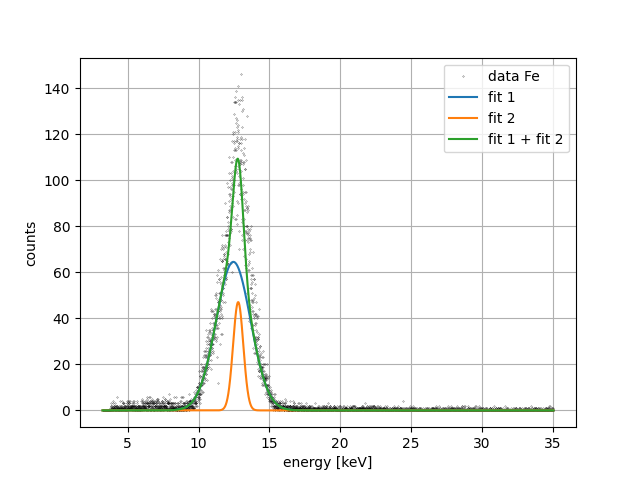
\includegraphics[width=110mm,scale=0.5]{MAX/include/plotsFe.png}
    \caption{spectrum and fit of Fe}
\end{figure}
\begin{figure}[H]
    \centering
    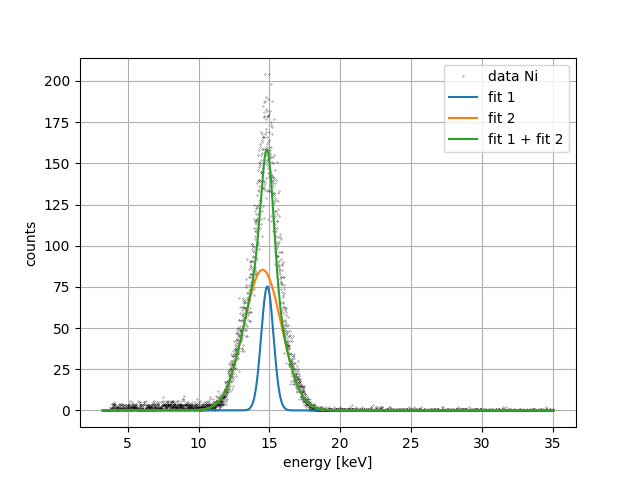
\includegraphics[width=110mm,scale=0.5]{MAX/include/plotsNi.png}
    \caption{spectrum and fit of Ni}
\end{figure}
\begin{figure}[H]
    \centering
    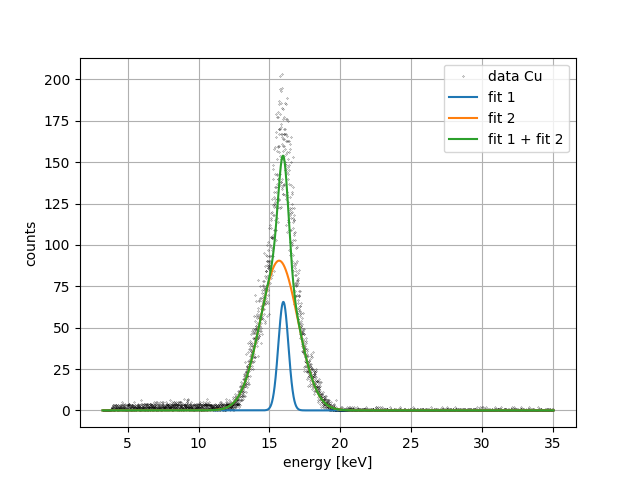
\includegraphics[width=110mm,scale=0.5]{MAX/include/plotsCu.png}
    \caption{spectrum and fit of Cu}
\end{figure}
\begin{figure}[H]
    \centering
    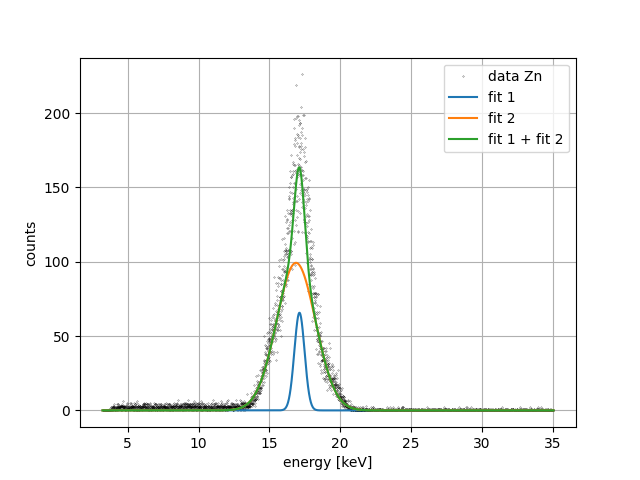
\includegraphics[width=110mm,scale=0.5]{MAX/include/plotsZn.png}
    \caption{spectrum and fit of Zn}
\end{figure}
\begin{figure}[H]
    \centering
    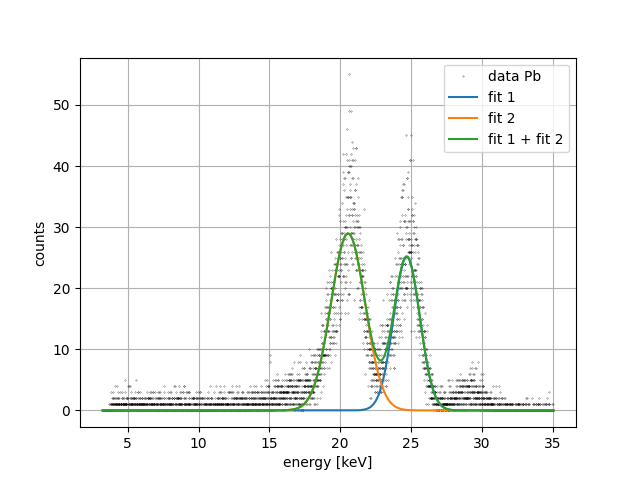
\includegraphics[width=110mm,scale=0.5]{MAX/include/plotsPb.png}
    \caption{spectrum and fit of Pb}
\end{figure}
